\normalfalse \difficiletrue \tdifficilefalse
\correctiontrue

%\UPSTIidClasse{11} % 11 sup, 12 spé
%\newcommand{\UPSTIidClasse}{11}

\exer{Suspension automobile  $\star\star$ \label{C2:07:55}}
\setcounter{numques}{0}
\UPSTIcompetence[2]{C2-07}
\index{Compétence C2-07}
\index{PFS}
\index{Suspension automobile}
\ifcorrection
\else
\textbf{Pas de corrigé pour cet exercice.}
\fi

\ifprof
\else
On s'intéresse à la liaison entre l'axe de la toue et le châssis du véhicule. Les notations adoptées seront les suivantes : $F^a_{C}$ (respectivement $F^r_{C}$, $F^x_{C}$) désignera la composante suivant $\vect{a}$ (respectivement $\vect{r}$, $\vect{x}$) de l'effort extérieur exercé en $C$. On procédera de même pour le point $D$. 
\begin{center}
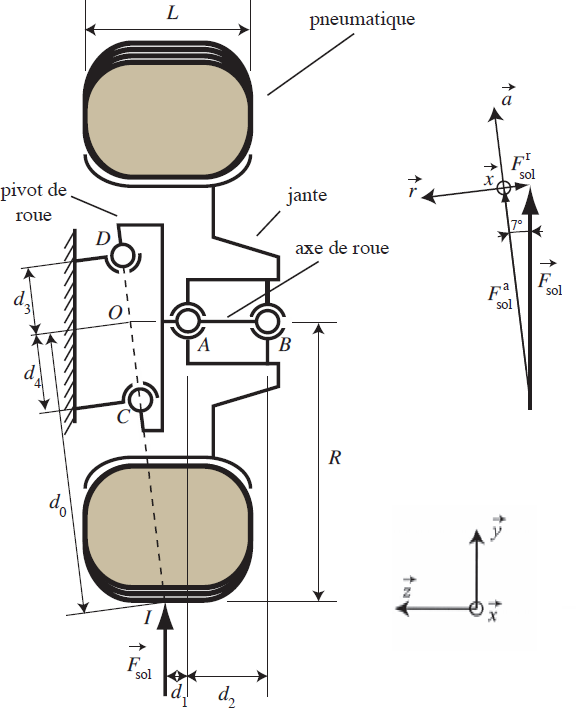
\includegraphics[width=\linewidth]{55_01}
\end{center}


\fi

\question{Réaliser le graphe des liaisons en faisant apparaître les actions mécaniques. Exprimer les torseurs des actions mécaniques de chacune des liaisons.}
\ifprof
\begin{center}
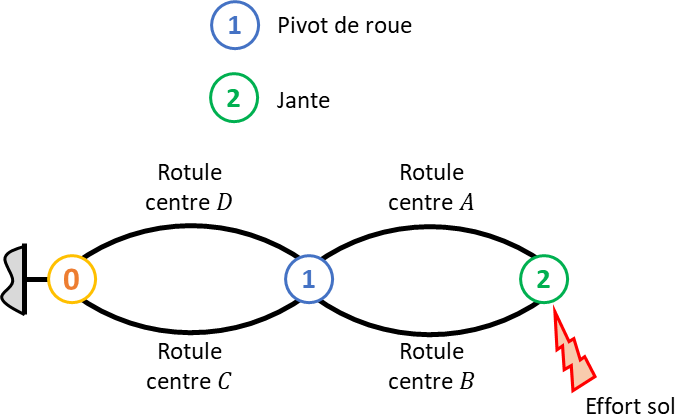
\includegraphics[width=10cm]{55_01_cor}
\end{center}

On a :
\begin{itemize}
\item $\torseurstat{T}{0}{1_C} =  \torseurl{X_C\vect{a}+Y_C\vect{r}+Z_C\vect{x}}{\vect{0}}{C}$;
\item $\torseurstat{T}{0}{1_D} =  \torseurl{X_D\vect{a}+Y_D\vect{r}+Z_D\vect{x}}{\vect{0}}{D}$;
\item $\torseurstat{T}{2}{1_A} =  \torseurl{X_A\vect{a}+Y_A\vect{r}+Z_A\vect{x}}{\vect{0}}{A}$;
\item $\torseurstat{T}{2}{1_B} =  \torseurl{X_B\vect{a}+Y_B\vect{r}+Z_B\vect{x}}{\vect{0}}{B}$.
\end{itemize}
\else
\fi

\question{En isolant l'ensemble \{pneumatique + jante + axe de roue\}, écrire les équations issues du principe fondamental de la statique appliqué au point $C$, en projection sur les axes de la base $\base{a}{r}{x}$ en fonction des composantes $F_{\text{sol}}^a$ et $F_{\text{sol}}^r$ et des dimensions $d_0$, $d_3$ et $d_4$.}
\ifprof

On isole l'ensemble demandé. 

BAME :
\begin{itemize}
\item $\torseurstat{T}{0}{1_C}$;
\item $\torseurstat{T}{0}{1_D} =  \torseurl{X_D\vect{a}+Y_D\vect{r}+Z_D\vect{x}}{\vect{0}}{D}$ 
$=  \torseurl{X_D\vect{a}+Y_D\vect{r}+Z_D\vect{x}}{ \left( d_4 +d_3 \right) Y_D \vect{x}-\left( d_4 +d_3 \right)  Z_D\vect{r}}{C}$
$\vectm{C}{0}{1_D}= \vectm{D}{0}{1_D} + \vect{CD}\wedge \vectf{0}{1_D}$
$= \left( d_4 +d_3 \right) \vect{a} \wedge \left( X_D\vect{a}+Y_D\vect{r}+Z_D\vect{x}\right)$
$= \left( d_4 +d_3 \right) \vect{a} \wedge  Y_D\vect{r}+\left( d_4 +d_3 \right) \vect{a} \wedge Z_D\vect{x}$
$= \left( d_4 +d_3 \right) Y_D \vect{x}-\left( d_4 +d_3 \right)  Z_D\vect{r}$.
\item $\torseurstat{T}{\text{Sol}}{2} =\torseurl{F_{\text{sol}}^a \vect{a}-F_{\text{sol}}^t \vect{r}}{\vect{0}}{I} $ 
$=\torseurl{F_{\text{sol}}^a \vect{a}-F_{\text{sol}}^t \vect{r}}{d_0F_{\text{sol}}^t \vect{x}}{C} $.
\end{itemize}

On applique le PFS en $C$ et on a : 

$$
\left\{
\begin{array}{l}
X_C + X_D + F_{\text{sol}}^a = 0\\
Y_C + Y_D - F_{\text{sol}}^t = 0\\
Z_C + Z_ D = 0 
\end{array}
\right.
\quad 
\left\{ 
\begin{array}{l}
0 = 0\\
-\left( d_4 +d_3 \right)  Z_D = 0 \\
\left( d_4 +d_3 \right) Y_D  + d_0F_{\text{sol}}^t= 0\\
\end{array}
\right.
$$

\else
\fi



\question{Résoudre littéralement le système.}
\ifprof
$$
\left\{
\begin{array}{l}
X_C + X_D + F_{\text{sol}}^a = 0\\
Y_C =- Y_D + F_{\text{sol}}^t \\
Z_C = 0 
\end{array}
\right.
\quad 
\left\{ 
\begin{array}{l}
0 = 0\\
  Z_D = 0 \\
 Y_D  = -  \dfrac{d_0F_{\text{sol}}^t}{d_4 +d_3}\\
\end{array}
\right.
$$

\else
\fi

\ifprof
\else
\ifcolle
\else
\footnotesize
\begin{enumerate}
\item .
\item .
\item $Z_C = Z_D = 0$, $ Y_D  = -  \dfrac{d_0F_{\text{sol}}^t}{d_4 +d_3}$, 
$Y_C =- Y_D + F_{\text{sol}}^t $.
\end{enumerate}
\normalsize
\fi
\begin{flushright}
\footnotesize{Corrigé  voir \ref{C2:07:55}.}
\end{flushright}%
\fi 